% !TeX spellcheck = ru_RU

\section{Эксперимент}

Для дальнейшего анализа производительности алгоритма были поставлены следующие задачи.
\begin{itemize}
    \item Замерить время работы реализаций на CPU и GPU и проанализировать типы запросов, работающих на GPU медленее, чем на CPU.
    \item Изучить масштабируемость реализации для GPU, сравнив время работы на двух разных по мощности тестовых стендах.  
\end{itemize}

\subsection{Условия эксперимента}
Эксперименты проводились на тестовом стенде со следующей конфигурацией.
\begin{itemize}
    \item \textbf{CPU}: Intel i5-10400f, 6 физических ядер, 12 потоков, максимальная частота 4.3 GHz
    \item \textbf{GPU}: Nvidia RTX 3050, 8 Gb VRAM, 1777 MHz
    \item \textbf{RAM}: 16 Gb, 3200 MHz, DDR4
    \item \textbf{OS}: Manjaro 6.14
    \item \textbf{Компиляторы}: nvcc 12.8, gcc 15.1
\end{itemize}
Измерялось только время работы алгоритма, загрузка входных данных в оперативную память и видеопамять не учитывалась.

В качестве данных была выбрана база знаний \textsc{Wikidata}\footnote{База знаний \textsc{WikiData}: \href{https://www.wikidata.org/wiki/Wikidata:Database_download}{https://www.wikidata.org/wiki/Wikidata:Database\_download} (Дата доступа: 19.06.2025)} \cite{wikidata}, на которой ставился эксперимент в предыдущей работе~\cite{PrevWork} и набор данных RPQ-bench\footnote{Набор данных \href{https://github.com/Mamenglu/LD-RPQB}{RPQ-bench} (Дата доступа: 19.06.2025)}.

\subsection{Анализ набора данных Wikidata}

Было проведено 15 измерений. Погрешность не учитывалась, так как стандартное отклонение не превышает 3\%.
Результаты измерения суммарного времени исполнения всех запросов представлены в таблице \ref{tab:ExpResults}.
Видно, что на Wikidata реализация на GPU выигрывает в производительности на 18\%, но проигрывает более чем в 3 раза на новом наборе данных RPQ-bench.

\begin{table}
    \centering
    \begin{tabular}{|c|c|c|c|}
\hline
Данные & Время GPU, \si{\second} & Время CPU, \si{\second} & Ускорение GPU \\
\hline
Wikidata & 115.73 & 136.30 & 1.18 \\
\hline
RPQ-bench & 185.28 & 55.19 & 0.30 \\
\hline
    \end{tabular}
    \caption{Результаты сравнения CPU и GPU}
    \label{tab:ExpResults}
\end{table}

Для визуализации результатов было составлено облако точек (Рис. \ref{fig:WikidataGraph}) с временем выполнения запросов на CPU и GPU. Видно, что среднее время выполнения запроса на GPU меньше, но медиана выше, так как на относительно маленьких запросах реализация на GPU, кроме самих вычислений, тратит значительную часть времени на синхронизацию.

Так же есть отдельные запросы, на которых алгоритм на GPU отрабатывает намного хуже. Ниже представлена таблица \ref{tab:worst4queris} с четырьмя запросами, на которых самый значительный проигрыш. 

\begin{table}[ht]
\centering
\caption{4 запроса, на которых GPU сильно проигрывает}
\label{tab:worst4queris}
\begin{tabular}{|c|c|c|c|c|}
\hline
№ запроса & Тип запроса & {Замедление} & {Время GPU, \si{\second}} & {Время CPU, \si{\second}} \\
\hline
132  & $(a^*~b^*)^+$ & 1.58   & 11.28  & 7.16  \\
\hline
443  & $a^*$ & 2.27   & 2.61   & 1.15  \\
\hline
207  & $(a\mid b)^+$ & 2.52   & 17.34  & 6.88  \\
\hline
% 67   & $((\widehat{\phantom{c}}\: a)~a)+$ & 43.05  & 9.04   & 0.21  \\
67   & $(~\hat{}a~a)^+$ & 43.05  & 9.04   & 0.21  \\
\hline
\end{tabular}
\end{table}

\begin{figure}[H]
    \centering
    \includesvg[width=\textwidth, pretex=\small]{figures/cloud.svg}
    \caption{Облако точек с временем выполнения запросов на GPU и CPU}
    \label{fig:WikidataGraph}
\end{figure}

Для трех запросов из таблицы \ref{tab:worst4queris} была обнаружена следующая закономерность --- у них очень большое количество ответов относительно соседних запросов, это можно заметить на Рис. \ref{fig:WikidataBadQueries}. Для 207 и 443 запроса видно, что у них количество ответов сильно превышает количество ответов у их соседей. Рядом же с 132-ым запросом есть 124-ый, у которого количество ответов даже больше, а работает он быстрее --- 6.60 секунд против 10.41 и вызывает замедление всего на 1.13, хотя все равно входит в пятерку самых долгих запросов. Для сравнения двух этих запросов было проанализировано количество итераций цикла --- 23 итерации у 124-го против 40 итераций у 132-го. Вероятно, столько времени 132-ой запрос тратит именно в дополнительных относительно 124-ого запроса итерациях.  

Для 67-го запроса эта закономерность не наблюдается. Был исследован тип этого запроса --- он представляется в виде $(~\hat{}a~a)+$, где $\hat{}$ обозначает разворот ребра. Но есть и другие запросы такого типа, например с 656 по 659, но в них значительного замедления не наблюдается.

\begin{figure}[H]
    \centering
    % 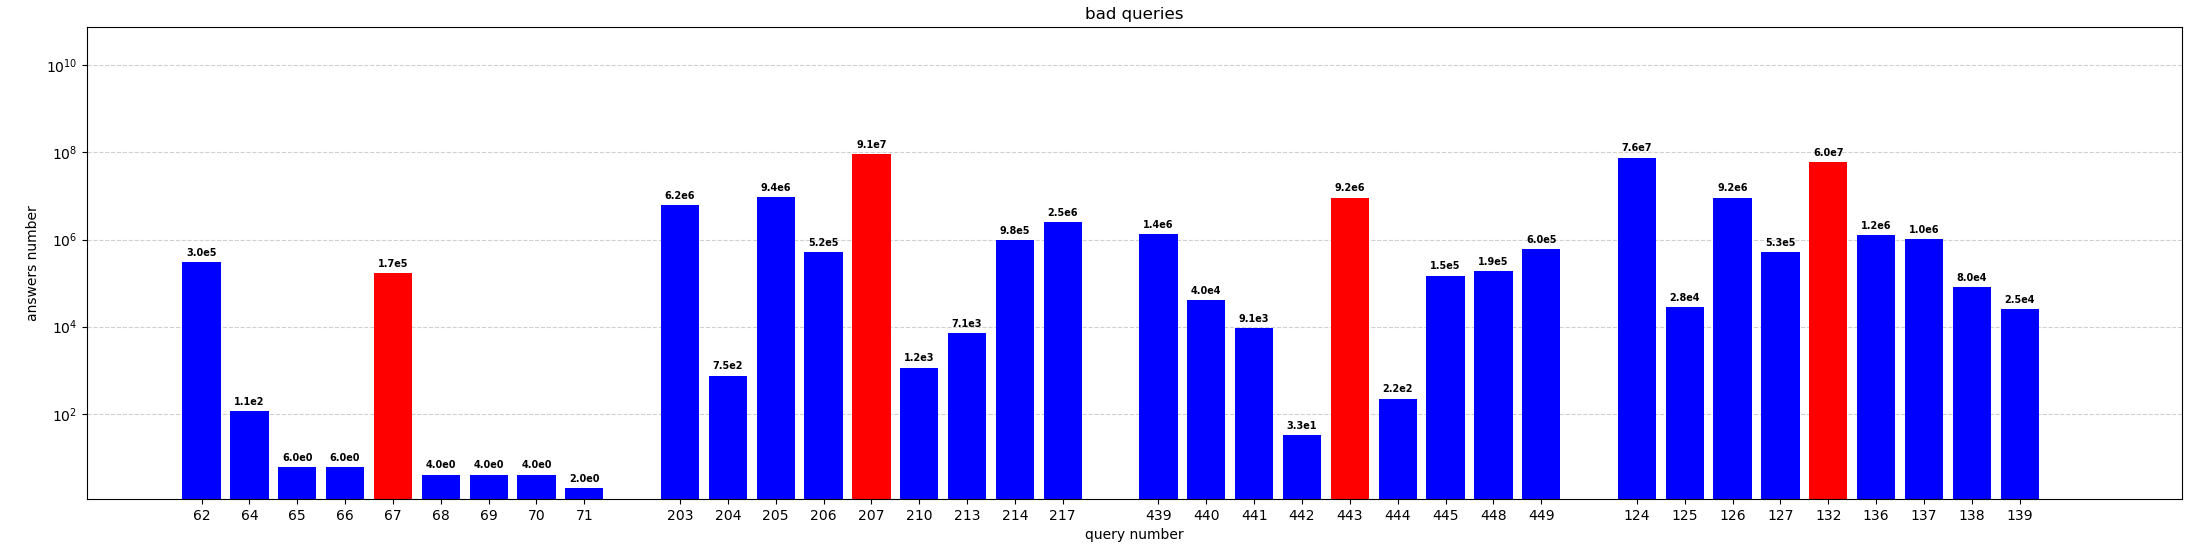
\includegraphics[scale = 0.36]{figures/answers.png}
    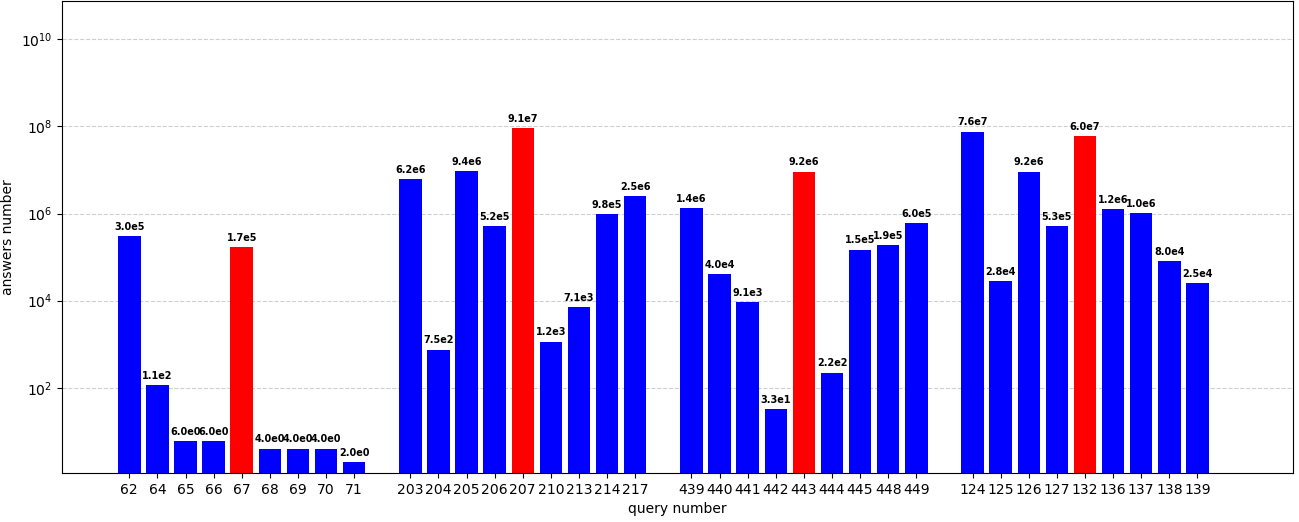
\includegraphics[width=\textwidth]{figures/answers_scaled.png}
    % 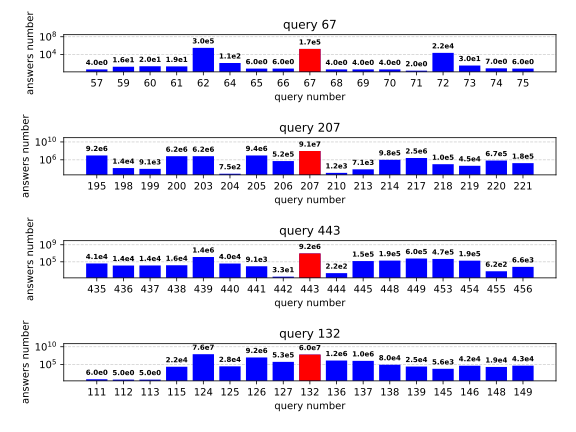
\includegraphics[scale = 0.36]{figures/worst.png}
    % \includesvg[width=\textwidth, pretex=\small]{figures/worst.svg}
    \caption{Столбчатая диаграмма, показывающая количество ответов у худших по ускорению  и ближайших к ним запросов. Худшие запросы выделены красным цветом.}
    \label{fig:WikidataBadQueries}
\end{figure}

\subsection{Анализ датасета rpqbench}

Для дальнейшего тестирования алгоритма был использован набор данных RPQ-bench\footnote{Набор данных \href{https://github.com/Mamenglu/LD-RPQB}{RPQ-bench} (Дата доступа: 19.06.2025)}.

Был создан набор данных на $10^7$ вершин и протестировано 20 типов запросов, для каждого типа было создано по 1000 запросов, то есть общее количество --- 20000.

Полное время работы на CPU составило 55 секунд, а на GPU --- 185.

Были проанализированы типы запросов: для каждого типа посчитано общее время выполнения, результаты представлены в таблице \ref{tab:rpqbench_types}. Можно заметить, что все типы запросов работают на GPU дольше, чем на CPU. Но соотношение 0.1 секунды на CPU и 3 секунды на GPU можно объяснить тем, что запросы этих типов достаточно малы, и их не стоит запускать на GPU, так как расходы на синхронизацию сильно превышают вычислительные расходы.
Интересно поведение GPU на типах запросов 11, 12 и 15, так как они значительно превышают остальные по времени работы.

\begin{table}[ht]
\centering
\caption{Типы запросов rpqbench}
\label{tab:rpqbench_types}
\begin{tabular}{|c|c|c|c|c|c|c|}
\hline
  № & Шаблон & Стартовая & Конечная & GPU, \si{\second} & CPU, \si{\second} & Замедление \\
\hline
  1  & $a b c$ & Любая & Фикс. & 3.61 & 0.10 & 34.40 \\
\hline
  2  & $a b c$ & Фикс. & Любая & 2.45 & 0.065 & 37.82 \\
\hline
  3  & $(a b c)\mid(c d d)$ & Фикс. & Любая & 4.31 & 0.13 & 33.30 \\
\hline
  4  & $(a b c)\mid(c d d)$ & Любая & Фикс. & 5.64 & 0.15 & 37.41 \\
\hline
  5  & $d^*$ & Фикс. & Любая & 2.68 & 0.072 & 37.15 \\
\hline
  6  & $d^*$ & Любая & Фикс. & 2.39 & 0.061 & 39.07 \\
\hline
  7  & $d^* e$ & Фикс. & Любая & 4.14 & 0.12 & 35.73 \\
\hline
  8  & $d^* e$ & Любая & Фикс. & 2.13 & 0.052 & 41.32 \\
\hline
  9  & $d^+$ & Фикс. & Любая & 2.61 & 0.07 & 39.19 \\
\hline
  10 & $d^+$ & Любая & Фикс. & 2.32 & 0.06 & 38.36 \\
\hline
  11 & $(a b)^*$ & Фикс. & Любая & 30.60 & 0.19 & 164.18 \\
\hline
  12 & $(a b)^*$ & Любая & Фикс. & 10.59 & 0.98 & 10.86 \\
\hline
  13 & $f g (d\mid e)$ & Фикс. & Любая & 38.54 & 16.49 & 2.34 \\
\hline
  14 & $f g (d\mid e)$ & Любая & Фикс. & 3.31 & 0.09 & 37.41 \\
\hline
  15 & $f g (d\mid e)^*$ & Фикс. & Любая & 45.92 & 35.34 & 1.30 \\
\hline
  16 & $f g (d\mid e)^*$ & Любая & Фикс. & 7.11 & 0.18 & 38.75 \\
\hline
  17 & $(c\mid g) (d\mid e)$ & Фикс. & Любая & 4.57 & 0.33 & 13.76 \\
\hline
  18 & $(c\mid g) (d\mid e)$ & Любая & Фикс. & 3.63 & 0.10 & 37.67 \\
\hline
  19 & $(c\mid g) (d\mid e)^*$ & Фикс. & Любая & 5.15 & 0.52 & 9.85 \\
\hline
  20 & $(c\mid g) (d\mid e)^*$ & Любая & Фикс. & 3.58 & 0.09 & 38.35 \\
\hline
\end{tabular}
\end{table}

На 15-ом типе CPU тоже работает долго, и в итоге замедление не очень значительное, его изучение с целью выявления слабых мест реализации на GPU не очень интересно. 11-ый и 12-ый тип запросов имеют одинаковый шаблон, различается только направление обхода графа --- в 12-ом типе все ребра графа развернуты в обратную сторону. Шаблон простой --- 2 ребра подряд под звездочкой Клини, и появилась гипотеза, что проблема в большом количестве итераций цикла поиска в глубину на стороне CPU, которая требует постоянной синхронизации с GPU. Для всех запросов было посчитано количество итераций и составлен поточечный график (Рис. \ref{fig:IterDep}), который подтвердил эту гипотезу.  

\begin{figure}[H]
    \centering
    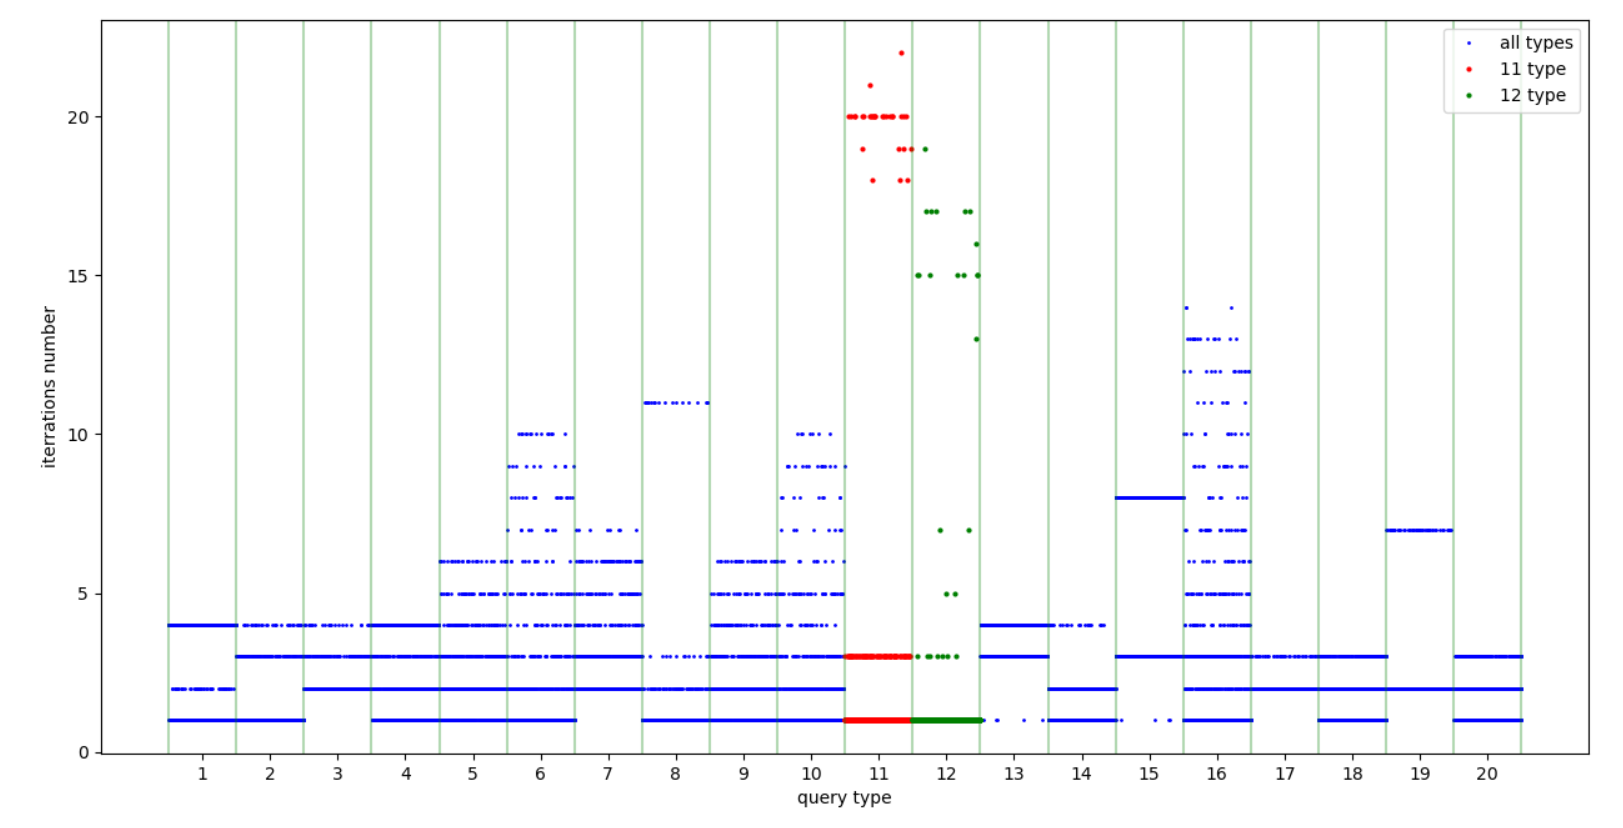
\includegraphics[scale = 0.4]{figures/iter_dep.png}
    % \includesvg[width=\textwidth, pretex=\small]{figures/itteration_number.svg}
    \caption{Количество итераций в каждом типе запроса}
    \label{fig:IterDep}
\end{figure}

% \begin{figure}[H]
%     \centering
%     \includegraphics[scale = 0.47]{figures/10kk-queries-types.png}
%     \caption{График общего времени исполнения каждого типа запросы}
%     \label{fig:QueriesTypes10kk}
% \end{figure}

% \begin{figure}[H]
%     \centering
%     \includegraphics[scale = 0.43]{figures/10kk-all-queris.png}
%     \caption{График времени работы для каждого запросов}
%     \label{fig:AllQueries10kk}
% \end{figure}

Анализ производительности в vtune показал (результаты представлены в таблице \ref{tab:RpqBenchVtune}), что время сложения и поэлементного умножения на инвертированную матрицу в реализации на GPU меньше, чем время этих операций на CPU (в LAGraph обе эти операции производятся через функцию \verb|GRB_assign|), время извлечения финальных вершин (функции умножения вектора на матрицу) больше в 3 раза, а вот время исполнения функции умножения в cuBool --- 178 секунд против 20 секунд в LAGraph --- почти в 9 раз больше. Можно сделать вывод, что для реализации на GPU узким местом является умножение матриц, то есть библиотека nsparse~\cite{Nsparse}. Со сложением матриц она уже показала, что не является оптимальным решением, возможно и произведение матриц тоже реализовано не оптимально.

\begin{table}[ht]
\centering
\caption{Время работы каждой операции на наборе данных rpqbench в реализациях на GPU и CPU}
\label{tab:RpqBenchVtune}
\begin{tabular}{|l|c|c|}
\hline
Операция & GPU, \si{\second} & CPU, \si{\second} \\
\hline
\centering
\verb|MxM| & 177.66 (78.93\%) & 20.37 (37.13\%)  \\
\verb|VxM| & 26.16 (11.62\%) & 8.08 (14.73\%) \\
\verb|cuBool_EwiseAdd| & 7.59 (3.37\%) & --- \\
\verb|cuBool_EwiseMulInverted| & 12.90 (5.73\%) & --- \\
\verb|GrB_Matrix_assign| & --- & 26.22 (47.79\%) \\
\hline
\end{tabular}
\end{table}

\newpage
\subsection{Анализ масштабируемости алгоритма}

% \footnote{Теоритическая \href{https://www.techpowerup.com/gpu-specs/geforce-rtx-3090.c3622#:~:text=Theoretical%20Performance}{мощность} RTX 3090.}
% \footnote{Теоритическая \href{https://www.techpowerup.com/gpu-specs/geforce-rtx-3050-8-gb.c3858#:~:text=Theoretical%20Performance}{мощность} RTX 3050.}
% \footnote{\url{https://www.techpowerup.com/gpu-specs/geforce-rtx-3090.c3622#:~:text=19.5%20Gbps%20effective-,Memory,-Memory%20Size}}
% \footnote{\url{https://www.techpowerup.com/gpu-specs/geforce-rtx-3050-8-gb.c3858#:~:text=14%20Gbps%20effective-,Memory,-Memory%20Size}}.

Для дальнейшего анализа реализации на GPU были проведены измерения с целью сравнения с предыдущими результатами  
на новом тестовом стенде со следующей конфигурацией.
\begin{itemize}
    \item \textbf{CPU}: AMD Ryzen 9 7900X, 12 физических ядер, 24 потоков, максимальная частота 5.733 GHz
    \item \textbf{GPU}: Nvidia RTX 3090, 24 Gb VRAM, 1692 MHz
    \item \textbf{RAM}: 128 Gb, 3600 MHz, DDR5
    \item \textbf{OS}: Ubuntu 24.04 LTS
    \item \textbf{Компиляторы}: nvcc 12.0, gcc 13.3
\end{itemize}

Теоретическая мощность RTX 3090 почти в 4 раза больше, чем у RTX 3050 --- 35.6 TFLOS против 9.2 TFLOPS, пропускная способность так же больше в 4 раза --- 936 Гб/c против 224 Гб/с.
Фактическая производительность, оценённая бенчмарком Passmark\footnote{\href{https://www.videocardbenchmark.net/compare/4284vs4495/GeForce-RTX-3090-vs-GeForce-RTX-3050-8GB}{Результаты} бенчмарка Passmark для RTX 3050 и RTX 3090 (Дата доступа: 19.06.2025)}, приблизительно в 2 раза больше.
Характеристики видеокарт взяты с сайта techpowerup\footnote{\href{https://www.techpowerup.com/gpu-specs/geforce-rtx-3050.c3858}{Характеристики} RTX 3050 (Дата доступа: 19.06.2025)}^{,}\footnote{\href{https://www.techpowerup.com/gpu-specs/geforce-rtx-3090.c3622}{Характеристики} RTX 3090 (Дата доступа: 19.06.2025)}.

Значит, если алгоритм хорошо масштабируем, то на RTX 3090 он должен работать хотя бы в 2 раза быстрее относительно на RTX 3050.

Так же, учитывая мощность RTX 3090, был создан набор данных rpqbench на $10^8$ вершин.

Результаты замеров представлены в таблице \ref{tab:Cmp305090}.

\begin{table}[ht]
\centering
\caption{Результаты замеров на RTX 3050 и RTX 3090}
\label{tab:Cmp305090}
\begin{tabular}{|c|c|c|c|}
\hline
Набор данных & RTX 3050, \si{\second} & RTX 3090, \si{\second} & Ускорение \\
\hline
wikidata & 116.50 & 100.99 & 1.15 \\
\hline
rpqbench $10^7$ & 185.28 & 131.46 & 1.41 \\
\hline
rpqbench $10^8$ & 318.86 & 300.17 & 1.06 \\
\hline
\end{tabular}
\end{table}

Интересно, что самое незначительное ускорение наблюдается на самом крупном наборе данных, хотя ожидалось обратное поведение. 

При помощи vtune было проанализировано, какую часть работы исполнения всех запросов на каждом наборе данных составляют функции cuBool, результаты представлены в таблице \ref{tab:MxMPart}. Можно заметить, что самую значительную часть составляет операция умножения. Именно в ней заключается проблема масштабирования --- она составляет большую часть времени, порядка 90\%, и работает на RTX 3090 примерно столько же, сколько и на RTX 3050, на остальных же функциях можно заметить значительное ускорение работы. 

\begin{table}[ht]
\centering
\caption{Время работы каждой операции на RTX 3050 и RTX 3090}
\label{tab:MxMPart}

Wikidata \\
\begin{tabular}{|c|c|c|c|}
\hline
Операция & RTX 3050, \si{\second} & RTX 3090, \si{\second} & Ускорение \\
\hline
\verb|MxM| & 92.99 (76.42\%) & 80.27 (79.99\%) & 1.16 \\
\verb|VxM| & 6.33 (5.20\%) & 1.67 (1.66\%) & 3.79 \\
\verb|EwiseAdd| & 16.90 (13.89\%) & 12.88 (12.84\%) & 1.31 \\
\verb|EwiseMulInverted| & 10.13 (8.32\%) & 5.53 (5.51\%) & 1.83 \\
\hline
\end{tabular}

rpqbench на $10^7$ вершин \\
\begin{tabular}{|c|c|c|c|}
\hline
Операция & RTX 3050, \si{\second} & RTX 3090, \si{\second} & Ускорение \\
\hline
\verb|MxM| & 177.66 (79.21\%) & 112.09 (84.55\%) & 1.58 \\
\verb|VxM| & 26.16 (11.66\%) & 8.58 (6.47\%) & 3.05 \\
\verb|EwiseAdd| & 7.56 (3.37\%) & 4.86 (3.67\%) & 1.56 \\
\verb|EwiseMulInverted| & 12.90 (5.75\%) & 7.04 (5.31\%) & 1.83 \\
\hline
\end{tabular}

rpqbench на $10^8$ вершин \\
\begin{tabular}{|c|c|c|c|}
\hline
Операция & RTX 3050, \si{\second} & RTX 3090, \si{\second} & Ускорение \\
\hline
\verb|MxM| & 274.71 (85.00\%) & 269.33 (90.27\%) & 1.02 \\
\verb|VxM| & 22.65 (7.00\%) & 11.22 (3.76\%) & 2.02 \\
\verb|EwiseAdd| & 15.28 (4.73\%) & 11.67 (3.91\%) & 1.31 \\
\verb|EwiseMulInverted| & 10.57 (4.27\%) & 6.15 (2.06\%) & 1.72 \\
\hline
\end{tabular}

\end{table}


